\chapter{绪论}
\section{研究背景与意义}

光学存储技术自20世纪80年代CD（Compact Disc）问世以来，历经DVD（Digital Versatile Disc）、Blu-ray（蓝光光盘）等技术迭代，凭借其非接触式读写、数据存储寿命长、单位存储成本低、抗电磁干扰等核心优势，在数据归档、影音传播、工业控制、航空航天等领域始终占据不可替代的地位。各领域数据呈爆发式增长，数据存储需求越来越大。根据数据的访问方式，可以将数据分为“热数据”和“冷数据”。“热数据”是指访问频率高的数据，需要存储在快速的存储设备上；“冷数据”是指访问频率低的数据，最好存储在更具成本效益的存储设备上。据IDC（International Data Corporation）预测，到2028年将产生393.8ZB（1ZB=1 万亿 GB）的数据，其中冷数据约占全部数据总量的60\%。这类数据对存储介质的稳定性、安全性和成本控制提出了极高要求，而光存储技术正是冷数据存储的核心解决方案之一。

\begin{figure}[h]
	\centering
	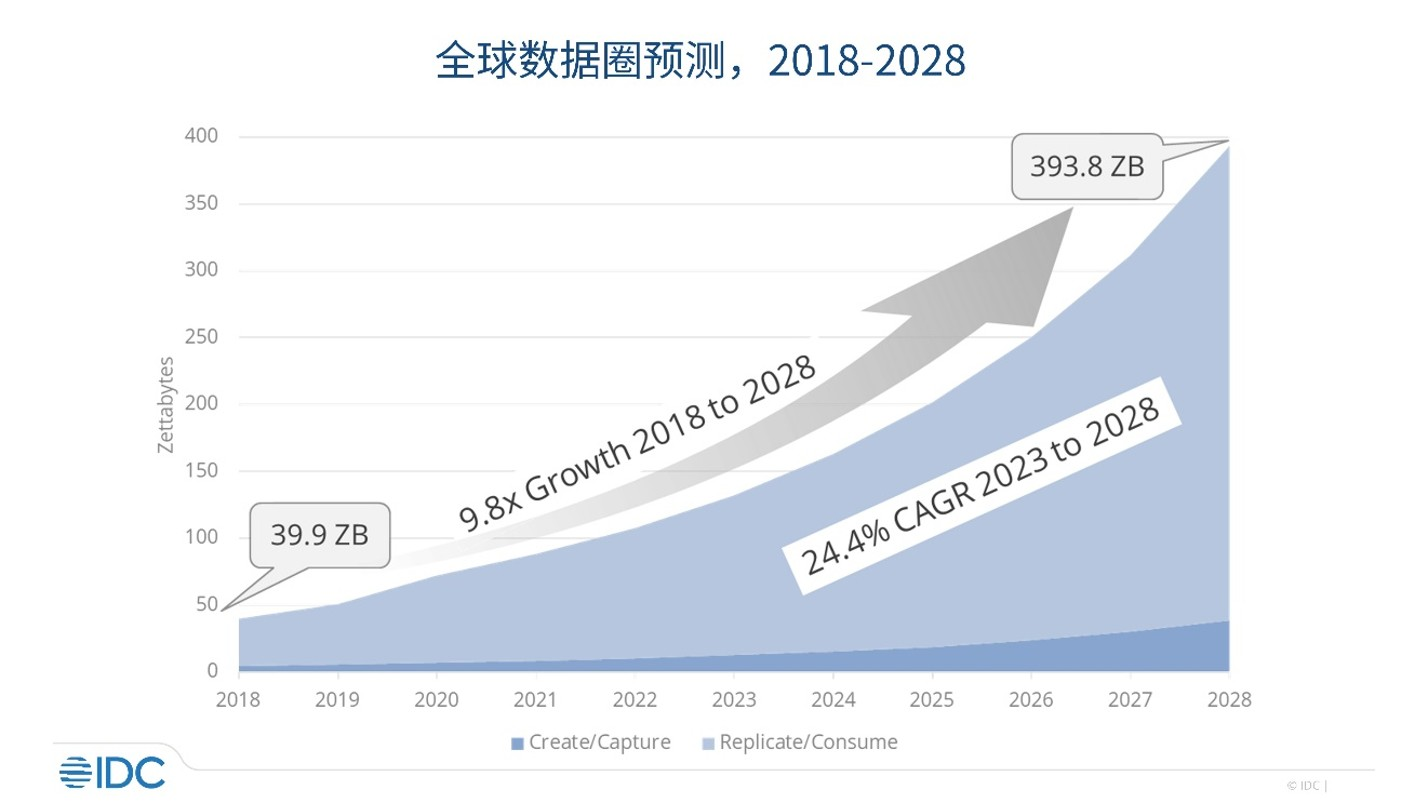
\includegraphics[width=0.8\textwidth]{float/ch.intro/idc.jpg}
	\caption{IDC全球数据预测图\label{fig:ch.intro.idc}}
	% \setlength{\belowcaptionskip}{-10pt}
\end{figure}

AD（Archival Disc）光盘作为新一代高密度光存储介质，其光盘英文名翻译过来就是“归档光盘”，从一开始就定位在数据归档存储领域，不考虑消费级市场的需求，其容量相对于BD光盘有显著提升。从行业实践来看，金融领域的合规要求直接凸显了冷数据存储的必要性与光存储的适配价值。根据金融监管标准\cite{Mifid2Data2018}，所有金融交易指令及执行记录需强制保存 7 年以上，且必须满足数据不可篡改（WORM）的合规性要求。典型案例显示，某跨地区银行在面临海量历史交易数据存储困境时，传统磁盘阵列方案不仅年运维成本高昂，且难以完全消除误删或篡改风险。通过引入融合蓝光光存储的智能分层存储方案，该银行将 90\% 的历史交易数据迁移至冷存储层，不仅使年存储总拥有成本（TCO）大幅降低，还充分利用了光存储介质的物理 WORM 特性，确保了审计时关键数据的真实性与完整性。

医疗领域同样离不开冷数据的可靠存储。单次 CT 检查产生的影像数据量可达 500MB，且根据医疗规范需保存 15 年以上\cite{MedicalImaging2024}。相关研究表明，相较于频繁出现物理损耗的硬盘阵列，光存储介质在 10 至 15 年的长期存储周期内具有极高的稳定性\cite{CTDataBackup2025}。某三甲医院改用光存储方案后，不仅解决了数据长期保存的稳定性难题，还依托光存储介质无需持续通电降温的特性，显著降低了年运维能耗成本，为基于历史病例开展 AI 辅助诊断研究提供了完整的数据基础。

在文化遗产保护与政务领域，冷数据存储的必要性与应用价值更为突出。某博物馆为实现文物数字化留存，采集了 TB 级文物高清影像数据。若采用传统介质，数据面临老化丢失风险且维护成本极高；通过光存储方案归档后，数据保存寿命可延长至百年级别，并有效抵御了电磁干扰对数字资产的影响。在政务档案管理方面，日本国家档案馆（NAJ）为实现档案数据的千年级留存，建立了基于 JIS Z6017 标准的可靠归档体系\cite{NAJ2020}。该体系选用的高稳定性蓝光光盘通过特殊材料工艺设计，验证了光存储在国家级冷数据存储场景中的核心作用，确保了政务数据在极端环境下的安全可读。

AD光盘的核心设计目标是突破传统蓝光光盘的存储密度瓶颈，其技术路线是在BD光盘基础上的升级，通过缩小轨道间距，提高记录密度大幅度提升了单盘容量，也提升了蓝光存储的综合竞争力。然而，随着存储密度的持续提升，AD光盘存储系统面临诸多技术挑战，尤其是由于衍射效应、码间干扰（Inter-Symbol Interference, ISI）、信道非线性以及噪声等因素引起的信号失真问题。这些问题严重制约了高密度光盘的读写性能与数据可靠性。为了提高光存储密度，近年来有多项新型光存储技术的研究，总体可分为两个思路：1、突破光学衍射极限，实现大幅度提高光存储密度和容量\cite{lzj2019}。2、维度复用，包括介质的三维空间，偏振，波长以及光强\cite{cwl2019}。本质上这些超高密度光存储技术是在物理材料层面上对光盘通道的改进，但随着信息记录密度越来越大，读写速度要求不断提高。这对光存储系统的读出系统的准确性提出了更高要求。

综上所述，在数据归档存储的实际应用中，如果能够有效解决高密度光存储中的信号失真问题，从而对读取信号进行精确恢复与均衡，就能在根本上保障归档数据的长期可读性与完整性，显著提升AD光盘作为冷数据存储核心介质的可靠性。因此，对光存储信道均衡与检测技术的研究显得尤为重要。而单纯依赖物理层面的存储密度提升（如突破衍射极限或多维复用）属于单向度的技术改进，难以系统性地应对由信道复杂性带来的综合性能挑战，因此本文结合AD光盘的高密度信道特性，对多通道自适应均衡技术进行深入研究，旨在为高可靠性的冷数据光存储系统提供关键技术支撑。


\section{国内外研究现状}
\subsection{光盘回读模型国内外研究现状}

光存储系统的读出通道（Read Channel）是实现高密度数据可靠提取的核心。自20世纪80年代CD技术问世以来，读出通道经历了几次重大的技术迭代。在早期CD和DVD阶段，由于记录密度较低，码间干扰（Inter-Symbol Interference, ISI）相对较轻，系统主要采用峰值检测（Peak Detection）和简单的阈值判定技术。随着存储密度的提升，尤其是蓝光（Blu-ray Disc, BD）以及新一代归档光盘（Archival Disc, AD）的出现，物镜数值孔径（NA）增大且激光波长缩短，导致光学衍射极限约束下的符号间距逼近物理极限。此时，严重的ISI使得传统的比特检测方式失效。为了应对这一挑战，读出通道演变为部分响应最大似然（Partial Response Maximum Likelihood, PRML）技术 \cite{braat2007diffractive}。PRML技术通过预设的部分响应（PR）目标（如PR(1,2,2,1)或PR(1,2,2,2,1)）来匹配读出信号的光学调制传递函数（MTF），并利用维特比（Viterbi）算法进行最大似然序列估计，极大地提升了高密度存储下的误码率表现。近年来，随着人工智能技术的兴起，基于神经网络的非线性均衡技术也开始被引入读出通道，以补偿高密度下的非线性失真。

在读出通道的设计与优化过程中，回读模型不仅是理论分析的基础，更是算法仿真与系统参数确定的核心工具。高精度的回读模型能够模拟激光束在微纳尺度坑点（Pits）或相变标记（Marks）上的散射过程，将物理层的光学信号转化为电子层的波形数据。

回读模型决定了通道均衡器（Equalizer）的设计上限，精确的模型可以预测由于盘片偏摆、离焦或球面像差产生的信号畸变；其次，它支撑了新型编码方案的有效性验证，避免了频繁制盘带来的研发成本；最后，随着多层存储和多维超分辨率存储技术的发展，物理模型必须能够准确描述层间串扰（Crosstalk）和非线性光学效应，否则读出通道将无法在极低信噪比环境下正常工作。

目前，学术界和工业界针对不同的存储密度和介质特性，开发了多种回读模型。

\textcolor{red}{以下可以再补充公式和图片以及参考文献}

\textbf{1. 基于衍射理论的模型（标量与矢量）}：
衍射理论是光存储回读的最经典模型。Braat等人 \cite{braat2007diffractive} 对此进行了详尽的综述，将模型分为标量衍射（Scalar Diffraction）和矢量衍射（Vector Diffraction）。
\begin{itemize}
	\item \textbf{标量模型：} 假设光波是标量场，适用于NA较小（如CD/DVD）的系统。Manfredonia在其研究中 \cite{manfredonia2007simulation} 利用标量理论仿真了短波长近场存储系统的读出信号。其优势在于计算效率极高，能快速生成海量均衡器训练数据，但其劣势在于无法处理高NA系统（如NA>0.85）中的偏振效应。
	\item \textbf{矢量模型：} 随着蓝光技术的发展，矢量衍射模型成为主流。Hermanus \cite{brusche2007mark} 建立了热-光学耦合的矢量模型，充分考虑了电磁波在微小坑点边缘的偏振分量变化。Jain等人 \cite{jain2022optimization} 进一步将矢量理论应用于多层蓝光光盘的读出优化，分析了多层介质中的能量衰减与偏振畸变。此类模型精度极高，但计算复杂度呈指数级增加。
\end{itemize}

\textbf{2. 复杂多维存储模型}：
针对更先进的存储架构，如多波束或超分辨率读写，模型需引入更复杂的物理变量。Liu等人 \cite{liu2022design} 提出了一种双光束读写配置方案，并利用改进的标量模型评估了多波束系统在不同轨道间距下的串扰抑制能力。研究表明，在多波束并行读出时，模型必须精确考虑波束间的干涉相消效应，以优化读出头的光学结构布局。

\textbf{3. 神经网络辅助的回读模型}：
近年来，国内外学者开始尝试利用深度学习构建“黑盒”回读模型。这类模型不再依赖复杂的波动方程，而是通过大量实测数据训练卷积神经网络（CNN）或循环神经网络（RNN）来拟合回读响应。其优点是能够自动捕获系统中难以建模的非线性噪声（如介质颗粒噪声），但在可解释性和外推性方面弱于基于物理理论的模型。例如，Wiecha 等人 \cite{wiecha2019pushing} 在研究中展示了如何利用深度卷积神经网络（CNN）突破光学信息存储的物理极限，通过对硅纳米颗粒散射光谱的端到端学习，该模型能够精确解码由于结构极度紧凑而产生的复杂光学信号，实现了对 4-bit 数据序列的无误码回读。

\subsection{光盘均衡技术国内外研究现状}

在信息存储阶段，用户数据经历了从电信号到光信号再到信息记录符的写入过程，如果要读出用户数据则需要完成以上过程的逆过程，这涉及编解码、写策略、信号采样、均衡检测等一系列步骤，其中，均衡（Equalization）环节可以有效降低噪声和串扰对有用信号的干扰，对于正确恢复用户数据有重要意义。其发展脉络与光盘记录密度的提升紧密相关。在 CD 与 DVD 的早期阶段，通道频带相对宽裕，主要采用线性均衡器。最初的实现方式是基于模拟滤波器的余弦均衡器，线性均衡器用来补偿信道非理想频率特性，减小抖晃、码间串扰，增大高频信号的幅值，提高过零检测的准确性。


\textcolor{red}{这里补充一个CD/DVD的通道图，以及对图的描述}


然而而随着光盘密度的提高，信息记录符也将越短，越短的信息记录符对应的信号频率越高，受到的抑制也就越严重。随着蓝光光盘的问世，这种均衡检测方案已经无法继续满足信号检测的误码率要求。于是研究者们提出了一系列新的均衡检测方法。早期蓝光系统中使用了限幅均衡系统，该系统能够在不增加符号间串扰的情况下改善信号高频成分\cite{bluray2015white}。在此基础之上，先锋公司综合考虑了多种均衡器的特点，提出了结构复杂的多均衡器联合均衡解决方案\cite{stek2002advanced}，这种方案将限幅均衡器、二维均衡器以及自适应均衡器分别用来补偿不同的干扰，虽然其表现出了很好的均衡性能，但是结构太过复杂且仅适用于三光束系统。进入高密度存储阶段后，为了应对紧凑记录符带来的严重 ISI。有研究者们借鉴 IBM 公司在磁存储中使用 （部分响应极大似然）PRML方法消除码间串扰的方式，将 PRML 法移植到了高密度光存储领域。

\textcolor{red}{这里补充一个PRML的通道图，以及对图的描述}

在基于PRML的高密度光盘存储系统里，Harumitsu Miyashita\cite{miyashita2002new} 等人提出了一种自适应均衡器，使用 LMS 算法处理不对称信号，提高了 PRML 信号处理的质量。Konako\cite{konakov2004high} 研究了用于光盘存储系统的混合模拟/数字 PRML 架构，通过结合数字和模拟电路，提高了数据检测的速度和效率。

PRML技术的出现，标志着光存储通道处理从“消除干扰”转向了“利用干扰”。在这一架构中，部分响应（Partial Response, PR）目标扮演着桥梁的角色。PR目标的作用在于将复杂的、具有无限冲激响应特征的光学信道，有意识地塑造成一种受控的、具有有限冲激响应特征的离散目标函数。Immink 与 Coene \cite{immink2004adaptation} 提出，PRML 的核心价值在于：它允许相邻符号之间存在可预测的重叠。通过均衡器将原始信号强制拟合至特定的 PR 目标，系统可以使用维特比（Viterbi）算法在格图（Trellis）上搜索最大似然路径。

\textbf{主流 PR 目标类型及其性能表征}
根据记录维度与密度的不同，研究者们开发了多种 PR 目标模型，并在实际系统中得到了广泛应用。

\textbf{1. 传统一维 PR 目标}
在一维高密度记录中，常用的目标包括 PR4、EPR4 以及针对蓝光优化的多项式目标。
\begin{itemize}
	\item \textbf{PR4 (1, 0, -1) 与 EPR4 (1, 1, -1, -1)：} Goss \cite{goss2006detection} 对这些目标在不同密度下的性能进行了对比研究。PR4 适用于中等密度，其优势在于格图状态数少，解码延迟低；而 EPR4 能够更好地匹配蓝光光盘的低通光学调制传递函数（MTF），在信噪比（SNR）增益上具有明显优势，但其代价是维特比译码器的计算复杂度呈指数级增加。
	\item \textbf{高阶多项式目标：} 针对归档光盘（AD），PR(1,2,2,2,1) 等目标被用于进一步压榨信道容量，使系统能有效处理更窄的脉冲响应。\textcolor{red}{这里再加一些专利里的PR}
\end{itemize}

\textbf{2. 二维与多维 PR 目标}
为了突破单轨道记录的极限，二维光存储（Two-DOS）技术应运而生。
\begin{itemize}
	\item \textbf{二维 PR0 模型：} Van Beneden \cite{van2008system} 在其博士论文中深入研究了二维光存储的系统表征。Immink \cite{immink2003signal} 提出了二维 PR0 目标，通过在空间维度（横向轨道与纵向比特）同时引入受控干扰，大幅提升了面密度。其优点是极大地缓解了轨道间串扰（ITD），但缺点是需要复杂的二维维特比检测算法，硬件实现成本极高。
	\item \textbf{多维优化策略：} Wang 等人 \cite{wang2014optimized} 针对多维光存储提出了一种优化的读取策略，通过定制化的 PR 目标检测，实现了多层介质中跨层干扰的有效分离，这为 3D 光存储的商业化提供了算法基础。
\end{itemize}

\textcolor{red}{还需要加一些近几年的文献}

\subsection{面临的关键问题}

随着光存储技术向更高密度、更大容量方向持续发展，AD光盘作为冷数据存储的核心介质，其读出信道面临着愈发严峻的技术挑战。尽管PRML技术已在蓝光及AD系统中得到广泛应用，显著提升了高密度下的数据恢复能力，但在追求极限存储密度的过程中，仍然存在以下问题：

\textbf{1.现有回读模型的精确度与实用性矛盾，制约了均衡器的优化上限。} 均衡器的设计严重依赖于对信道特性的精确建模。更高密度的盘片要求更准确的回读模型。

\textbf{2.单一均衡通道难以协同处理复杂多维干扰，尤其是轨道间串扰（ITI）。} 即使拥有一个相对准确的模型，传统的单通道均衡架构也难以应对高密度信道的复合干扰。除了由衍射和信道带宽限制引起的一维码间干扰（ISI）外，窄轨距带来的二维轨道间串扰（ITI）已成为提升面密度的核心瓶颈。

\textbf{3.系统在动态环境下的鲁棒性与自适应能力亟待提升。} 高密度存储下信号幅度微弱，系统对各类噪声（介质噪声、电子噪声等）异常敏感。同时，在实际归档场景中，光盘的长期老化、不同驱动器间的性能差异，都要求读出通道具备强大的环境自适应能力。然而，当前多数均衡算法（如LMS）的参数更新机制在低信噪比或信道突变时易出现误差传播、收敛缓慢甚至发散的问题。更根本的是，当信道变化超出了均衡器预设的线性或有限非线性补偿范围时（例如因盘片严重翘曲导致的强烈非线性畸变），任何基于固定PR的均衡器都可能失效。


\section{研究内容与创新点}
本文面向高密度归档光盘（AD）存储系统，聚焦于提升其读出信号处理链路的性能与可靠性。针对当前AD光盘信道均衡技术所面临的回读模型失配、干扰复杂以及目标响应固定等关键问题，本文提出了一套系统的解决方案。研究内容遵循“精确建模—高效均衡—动态优化”的技术路线，旨在构建一个更精准、更稳健、更自适应的信号处理框架。核心研究内容与创新点如下：

\begin{figure}[h]
	\centering
	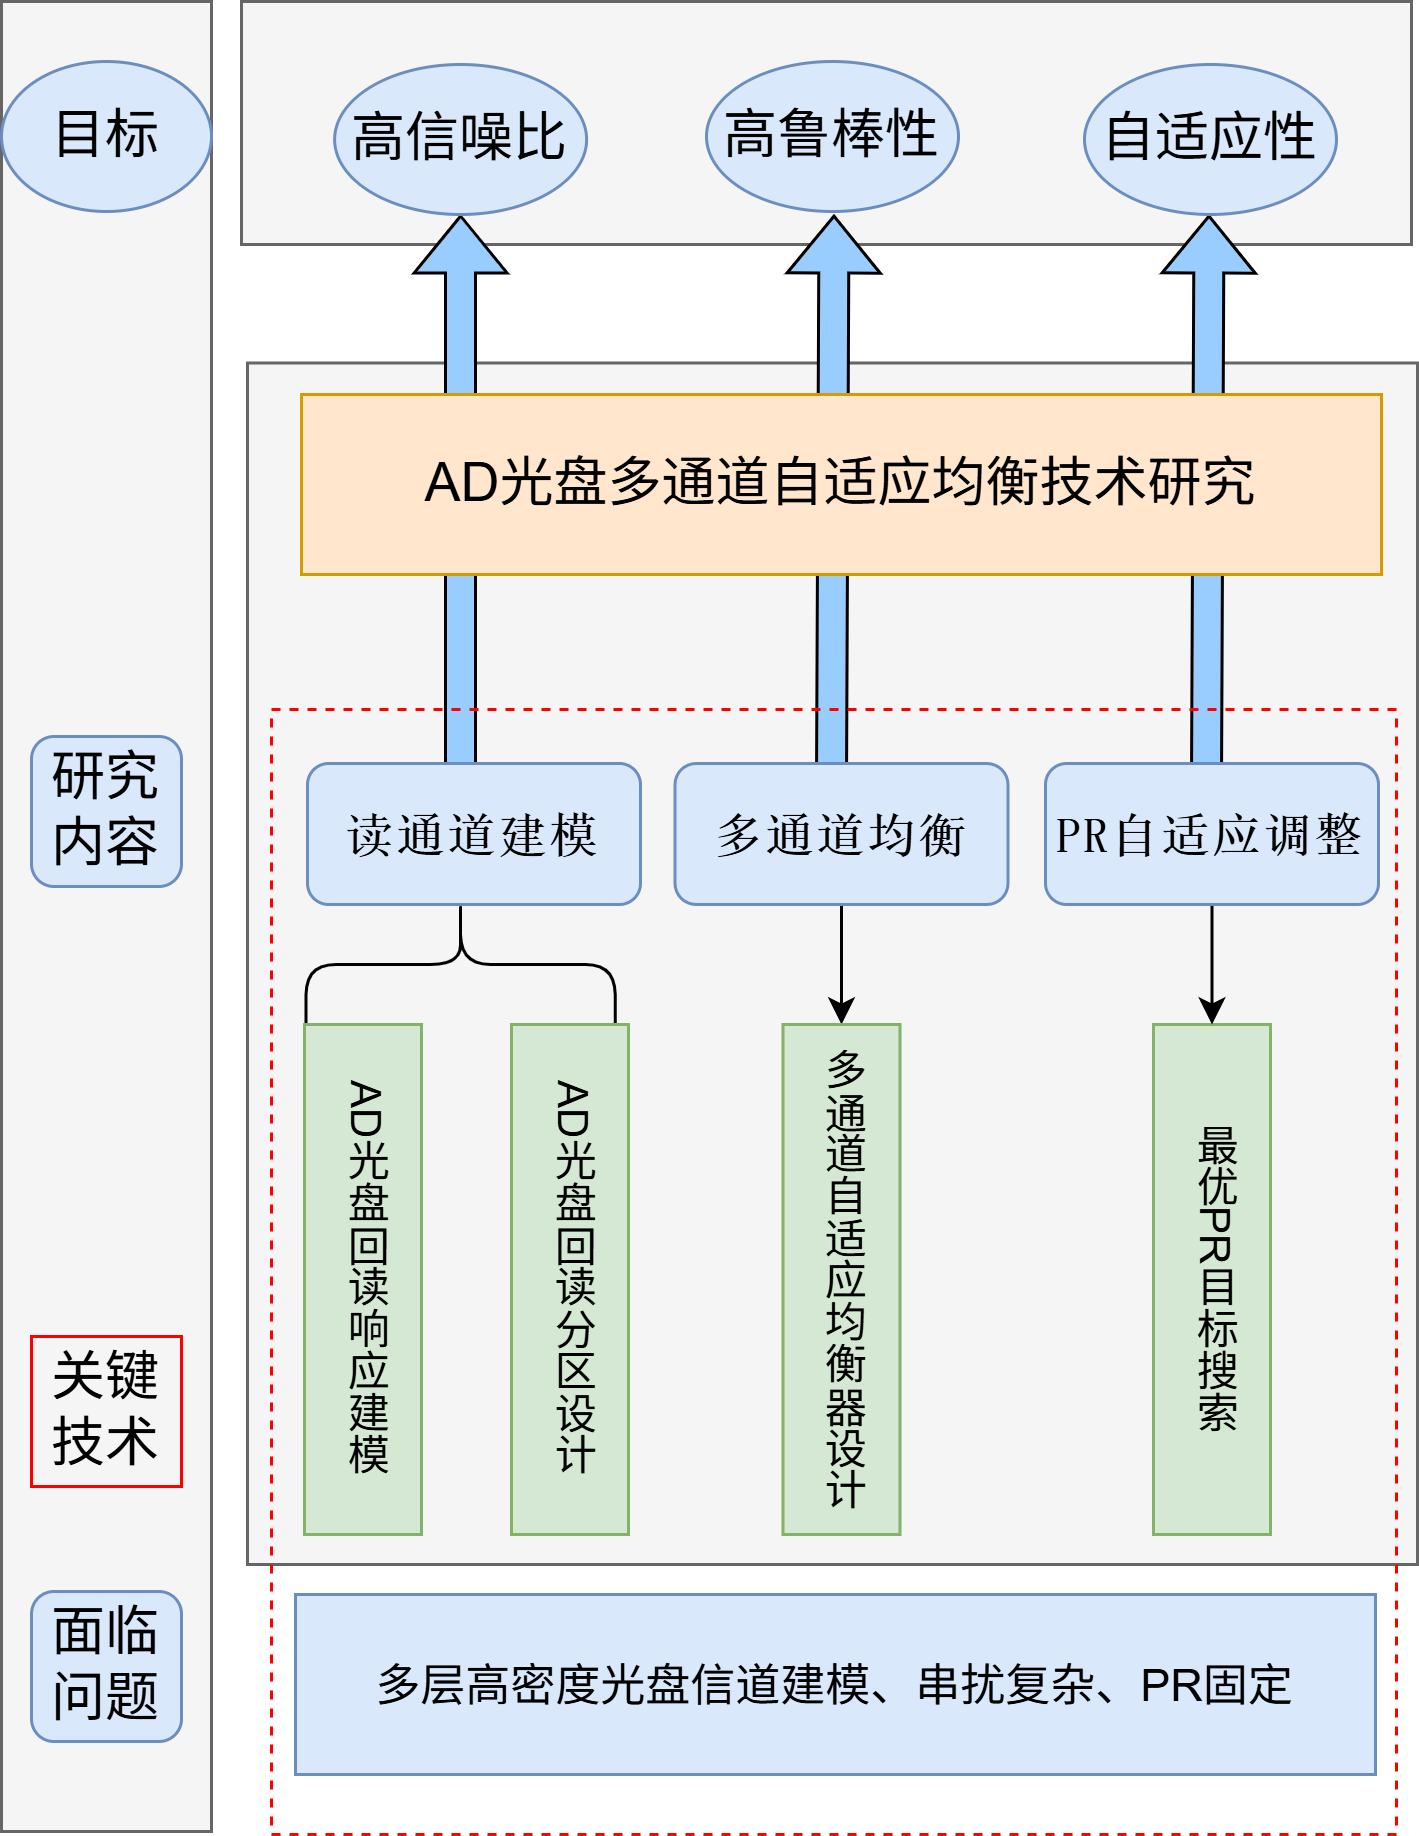
\includegraphics[width=0.8\textwidth]{float/ch.intro/maincnn.png}
	\caption{本文主要研究内容\label{fig:ch.intro.maincnn}}
	% \setlength{\belowcaptionskip}{-10pt}
\end{figure}

本文的主要工作与创新点如下：

1. \textbf{构建高精度分区化回读信道模型}。依据AD光盘的记录符（Mark）尺寸、激光波长、轨道间距等基础信道参数，在点扩散函数（PSF）光盘读出模型[33]的基础上，提出一种多分区差异化建模方法。该模型将光盘信道按物理与信号特征划分为多个子区，并针对各分区构建适配的简化响应函数，从而生成更贴合实际、更具区分度的回读信号样本，为后续均衡器设计与训练提供精准可靠的信道先验知识。

2. \textbf{设计基于多通道协同的自适应均衡架构}。针对高密度信道中码间干扰（ISI）与轨道间串扰（ITI）等多维干扰耦合的问题，提出一种基于LMS的多通道并行处理与动态融合均衡新架构。该架构通过构建多个分别优化于特定干扰抑制的均衡通道，并引入通道输出权重在线分配机制，实现了对复合干扰的协同抑制。同时，该架构建立了部分响应（PR）目标与实时信道状态信息（如信噪比、均衡误差）间的动态映射关系，为系统在不同干扰条件下的最优检测模式切换提供了结构基础。

3. \textbf{提出基于智能搜索的动态PR目标优化策略}。为解决固定PR目标难以适应信道时变性与非线性变化的问题，首次将人工蜂群（ABC）优化算法引入光存储均衡领域，提出一种轻量级在线最优PR目标搜索方法。该方法以均衡器均方误差为适应度函数，驱动ABC算法在预设的PR目标候选库中进行高效寻优，动态选取或微调出与当前信道条件最匹配的PR多项式。该策略显著提升了系统在信道漂移、盘片差异及长期老化等动态环境下的自适应能力与检测鲁棒性。

\section{论文组织结构}

\textcolor{red}{这个要重新组织一下，不能抄目录}
本文围绕“AD光盘多通道自适应均衡技术”这一主题展开，各章具体内容安排如下：

\textbf{第一章}

阐述研究背景与意义。首先，从冷数据存储的刚性需求出发，论述了高密度光存储在数据归档领域的核心价值与AD光盘面临的挑战。其次，系统梳理了光盘回读模型与均衡技术的国内外研究现状，凝练出当前技术面临的关键问题。最后，明确本文的研究目标、主要研究内容与创新点，并给出全文的组织结构安排。

\textbf{第二章：基于分区信道建模的均衡信号生成}

本章针对回读模型信号区分度不足的问题，提出解决方案。首先，分析传统均匀信道模型在高密度条件下的局限性。接着，详细阐述基于点扩散函数（PSF）的多分区建模方法，包括分区策略、各分区简化响应函数的构建过程。最后，通过仿真实验，验证所提模型在信号匹配精度和计算效率方面的优势，并与传统模型进行对比分析。

\textbf{第三章：基于多分区的自适应均衡器设计}

本章致力于解决多维干扰协同抑制的难题。首先，提出多通道并行均衡的系统架构。其次，阐述基于LMS算法的通道自适应更新。最后，设计仿真实验，评估该均衡架构在典型高密度信道下对信噪比（SNR）的提升效果及对复杂干扰的抑制能力。


\textbf{第四章：基于PR目标的均衡优化系统}

本章聚焦于提升系统的自适应性与鲁棒性。首先，提出基于人工蜂群（ABC）算法的最优PR目标在线搜索策略，详细说明适应度函数设计、搜索流程与切换逻辑。其次，构建完整的“模型-均衡-检测”闭环系统仿真平台。最后，通过多组对比实验，综合评估系统在静态、动态及存在模型失配等多种场景下的误码率（BER）性能，验证本文所提方案的有效性与先进性。

\textbf{第五章：总结与展望}

总结全文的研究工作与主要结论，归纳本研究在理论方法和技术应用上的贡献。同时，客观分析当前研究存在的局限与不足，并对未来在模型泛化能力、硬件实现架构以及与其他先进信号处理技术融合等方面可能的研究方向进行展望。
